\chapter{Methodology}
\label{chapter:prop}

\section{Proposal}

In this chapter, we propose our plan and schedule to achieve the goals of building a \ac{ser} system, integrating another modality, and evaluating its effectiveness in a video conference context. Figure \ref{fig:gantt} illustrates our research plan and schedule through a Gantt chart.

\begin{figure}[h]
	\centering
	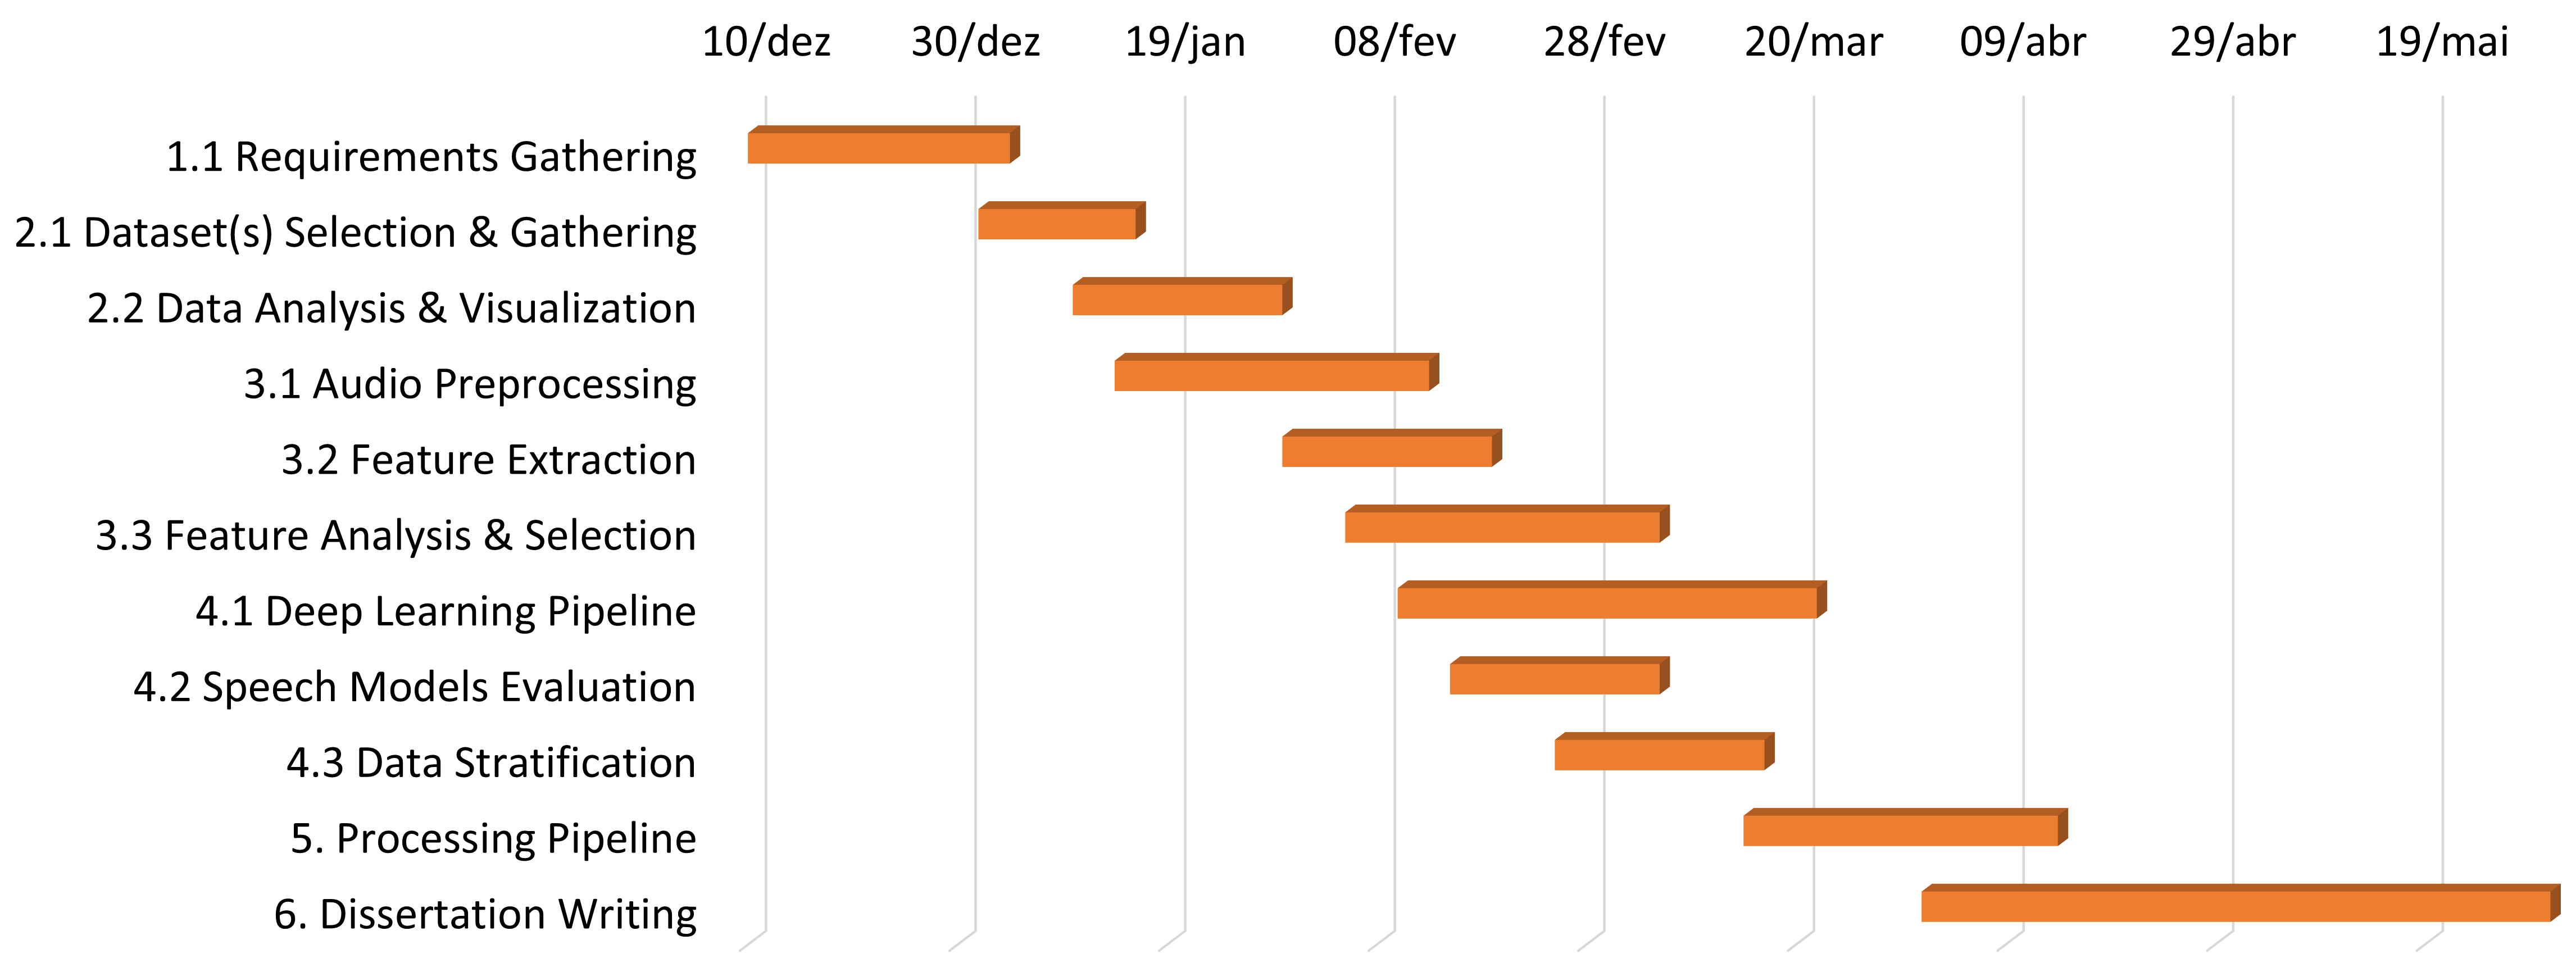
\includegraphics[width=\linewidth]{figs/3_methodology/gantt_chart.png}
	\caption{Gantt chart with the proposed work plan for this research.}
	\label{fig:gantt}
\end{figure}

\subsection{Requirements Gathering}

Initially, we conducted a requirements-gathering process to understand the needs, expectations, and constraints of our emotion recognition system. We identified specific use cases in which the system would be applied, and from there we were able to determine various requirements, including ethical considerations and technical requirements. These requirements served as the foundation for our defined objectives and strategies.


\subsection{Dataset}

\subsubsection{Dataset(s) Selection \& Gathering}

The next step is the selection of one or more audiovisual datasets that, in line with the \ac{sota} research, are preferably large and diverse (e.g., by featuring individuals of both genders, different scripts, contexts, etc.).

\subsubsection{Data Analysis \& Visualization}

Data analysis and visualization will allow us to explore, understand and display the data. Using various techniques such as statistical analysis, machine learning, and computational methods, we aim to extract information and then create graphical representations of it, in a way that allows us to better understand the dataset. 

\subsection{Audio Feature Engineering}

Once the dataset(s) have been selected, following the traditional feature-based approach, audio feature engineering will be required. In the context of machine learning, audio feature engineering involves preprocessing, extracting, and selecting relevant features from audio signals to build effective systems.

\subsubsection{Preprocessing}

\paragraph{Framing}

Speech framing, also called signal segmentation, is the process of dividing continuous speech signals into fixed-length segments. Speech typically stays consistent for a relatively short period, such as 20 to 30 ms. By dividing the speech signal into frames, local features can be extracted. Additionally, the relationship and information between the frames can be preserved by deliberately overlapping 30\% to 50\% of these segments. After creating the speech frames, researchers often apply a windowing function to smooth the edges and improve the time-frequency resolution of the signal \cite{Akay2020}.

\paragraph{Noise reduction}

Noise can have a significant negative impact on the quality of an audio signal by masking or distorting important features of the speech. It can also introduce variability into the audio data, making it harder for the machine learning model to generalize to new situations. The most successful methods for noise reduction are the Minimum Mean Square Error (MMSE) and Log-spectral Amplitude MMSE estimators \cite{Pohjalainen2016}.

\paragraph{Normalization}

Scale differences in features' values may affect the models' performance, especially those based on distance metrics to parameter estimation. So, it is advised to normalize features to prevent this effect. This can lead to more accurate and consistent results when applying the model to new data. The most widely used normalization techniques are z-normalization (also known as standardization) and min-max normalization \cite{Akay2020}.

\paragraph{\acl{vad*}}

\ac{vad*} is a technique used in speech processing to identify periods of speech in an audio signal. By focusing on analyzing the voiced speech and ignoring noisy or silent periods, \ac{vad*} can improve the accuracy of a system by reducing the influence of non-speech segments on the analysis. Furthermore, it can decrease the computational cost by reducing the amount of data to be processed. Commonly used methods for \ac{vad*} include zero crossing rate, short-time energy, and auto-correlation \cite{Akay2020}.

Figure \ref{fig:vad} demonstrates an instance where a \ac{vad*} system is applied to a speech signal, in this case, it is processing chunks with a duration of 1 second. It reduces the original signal of 10 seconds by half by identifying 5 voiced segments that are then fed to a \ac{ser} model \cite{Milling2022}.

\begin{figure}
	\centering
	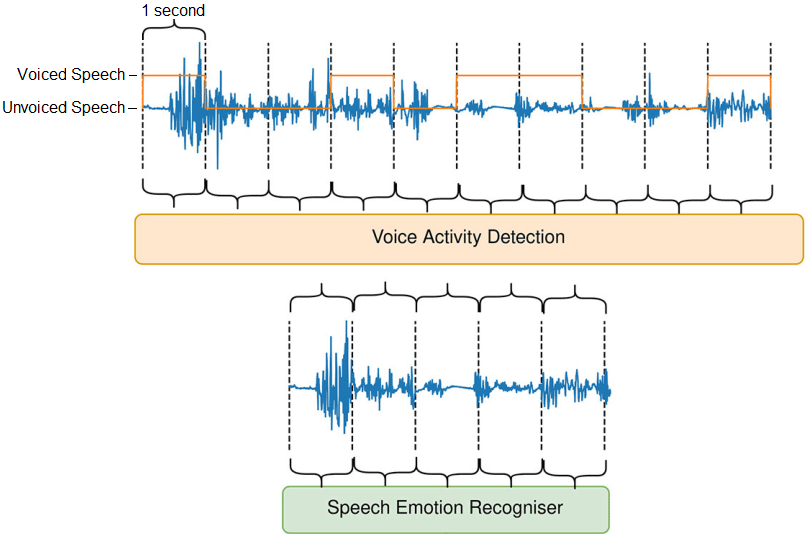
\includegraphics[width=.8\linewidth]{figs/3_methodology/speech_activity_detection.png}
	\caption{\acl{vad*} employment on an audio signal \cite{Milling2022}.}
	\label{fig:vad}
\end{figure}


\subsubsection{Feature Extraction}

Various techniques can be used to extract features from audio signals, such as time-domain analysis, frequency-domain analysis, and signal processing algorithms. These techniques can be used to extract features such as spectral features, temporal features, and statistical features. When studying the features extracted from speech audio signals, it is common to consider both global and local features \cite{PORIA201798}. Some emotions are more prominent at the beginning or end of a speech, so it is frequent to consider both global and local features to fully capture the temporal and emotional content of the signal.

\subsubsection{Feature Selection}

In order to achieve optimal performance, it is important to carefully select the features used in any model. Including redundant or uninformative features can degrade performance. By selecting and reducing the number of features, it is possible to maintain or even improve performance while using fewer resources and avoiding overfitting, also it becomes easier to understand the model's decision-making process and which features are most important.

\subsection{Models Implementation}

\subsubsection{Deep Learning Pipeline}

In addition, we will experiment and compare the effectiveness of automatic audio feature extraction-based approaches to \ac{ser}, using either the raw audio signals, \ac{mfccs}, or Mel spectrograms as input to deep learning models, some transfer learning techniques will also be explored.

\subsection{Speech Models Evaluation}

After we have chosen the relevant features through the feature selection process and completed the deep learning pipeline, we will test various models, and measure their performance by using appropriate metrics, to then identify the best classifiers for the traditional feature-based and \ac{dl}-based approaches.


\subsection{Data Stratification}

Data stratification refers to a process of dividing a dataset into subgroups, based on certain properties. We will test different ways of grouping the labeled data and interpreting their effects on the model's predictions, for example, by relabeling the angry and sadness samples as \textit{negative} samples. By doing this, we can discover potential biases in both the classifiers and the dataset(s), such as the individual's age, gender, and even the evaluation of the samples given by juries.


\subsection{Deployment}

\subsubsection{Processing Pipeline}

The most suitable model for offline and online scenarios will be analyzed and tested in a real-time scenario using an audio segmentation pipeline with \ac{vad*}.

\subsection{Dissertation Writing}

To conclude the work plan, we will focus on a comprehensive discussion of our research, including any potential challenges and limitations that we encountered and the steps we took to address them.

\section{Ethical Procedures and Concerns}

There are several ethical concerns when building emotion recognition systems, and in our case, we will address those related to \ac{ser} systems. One of them is that they may not be accurate in recognizing emotions for people with certain characteristics (age, gender, accents, speech disabilities, etc.), which is why we will address and quantify some potential biases in our models.

Another concern is that these systems may be used to monitor or control persons without their consent. Our models will only be in use on individuals that fully consented to submit their data for emotional evaluation purposes.

Additionally, there may be privacy concerns about personal data collected by these systems being vulnerable to hacks or used for unintended purposes. Our processing pipelines will only utilize the participant's streaming data for the \ac{ser} models input, and, will not store or use the sensitive data for any other purposes than the emotional analysis. We also decided to not use speech transcriptions, as it raises even greater privacy issues, due to capturing the actual words spoken and can reveal confidential data such as personal, financial, or business information.

In summary, we intend to be transparent about the system's capabilities and limitations and obtain informed consent before collecting and using any personal data.

